\section{A controlled linear-stability test}
\label{sec:stability}
The source states that resolving counter-streaming populations allows its
two-fluid model to capture the linear growth of the associated
instabilities~\cite{original}. Population resolution alone does not guarantee
the correct kinetic response. Closure-dependent differences in fluid and kinetic
instability spectra are established issues~\cite{ng2019,wang2015}. We give an
explicit test of the stated local-isotropization closure, without inferring
that the test mode occurs in the source's nonlinear reconnection calculation.

Consider a homogeneous nonrelativistic electron plasma with immobile
neutralizing ions. Two equal-density populations have ordinary velocities
$\pm Ue_x$ and isotropic thermal variance $\sigma^2$. Their longitudinal
velocity marginal, normalized to unit density, is
\begin{equation}
 f_0(v)=\frac{
 e^{-(v-U)^2/(2\sigma^2)}+e^{-(v+U)^2/(2\sigma^2)}
 }{2\sqrt{2\pi}\sigma}.
 \label{eq:kinetic-equilibrium}
\end{equation}
A constant magnetic field parallel to $e_x$ leaves the longitudinal,
gyrotropic perturbation subspace used below invariant.

\paragraph{The collisionless kinetic reference.}
For $U>\sigma$, the only local minimum of $f_0$ is at zero. Indeed,
$f'_0/f_0=[-v+U\tanh(Uv/\sigma^2)]/\sigma^2$, and
$U\tanh(Uv/\sigma^2)-v$ is strictly concave on $v>0$, with exactly one
positive zero. The Penrose criterion~\cite{penrose1960} therefore tests
\begin{equation}
 I=\int_{\R}\frac{f'_0(v)}v\,\dd v
 =\frac{2\zeta D(\zeta)-1}{\sigma^2},
 \qquad
 \zeta=\frac{U}{\sqrt2\sigma},\quad
 D(z)=e^{-z^2}\int_0^z e^{t^2}\,\dd t.
 \label{eq:penrose-integral}
\end{equation}
This integrand has a removable singularity at zero. At $U/\sigma=6/5$,
$\zeta^2=18/25$. The alternating Dawson series has decreasing term magnitudes
and gives the rational upper bound
\begin{equation}
 2\zeta D(\zeta)
 \leq \frac{36}{25}-\frac{432}{625}+\frac{15552}{78125}
 =\frac{74052}{78125}<1.
 \label{eq:penrose-rational}
\end{equation}
Consequently $I<0$, and this kinetic equilibrium has no exponentially growing
longitudinal electrostatic mode for any real wavenumber. Direct quadrature gives
$\sigma^2 I=-0.08730405848\ldots$; the sign does not depend on that numerical
evaluation.

\paragraph{Linearizing the finite-relaxation fluid model.}
The source retains
$\partial_mq_{sijm}=\nu(p_{sij}-\delta_{ij}\tr p_s/3)$,
with $\nu=\kappa\sigma>0$. Normalize the total plasma frequency, density,
electron mass, charge magnitude and permittivity to one. For each beam
$s=\pm$, set $U_s=sU$, $n_s=1/2$, and equilibrium diagonal pressure
$p_s^0=n_s\sigma^2$. Write its perturbations as
$N_s=\delta n_s$, $V_s=\delta u_{sx}$,
$P_s=\delta p_{sxx}$ and $H_s=\delta\tr p_s$.
For spatial factor $e^{ikx}$, the invariant nine-variable system is
\begin{align}
 \dot N_s&=-ikU_sN_s-ikn_sV_s, \nonumber\\
 \dot V_s&=-ikU_sV_s-ikP_s/n_s-E, \nonumber\\
 \dot P_s&=-ikU_sP_s-3ikp_s^0V_s-\nu(P_s-H_s/3), \nonumber\\
 \dot H_s&=-ikU_sH_s-5ikp_s^0V_s, \nonumber\\
 \dot E&=\sum_{s=\pm}(U_sN_s+n_sV_s).
 \label{eq:linear-block}
\end{align}
Here $\delta p_{syy}=\delta p_{szz}=(H_s-P_s)/2$. A perturbation of $\nu$
multiplies the zero equilibrium deviator and thus contributes nothing at
linear order, even when thermal speed is computed locally.
Eliminating these variables independently, with temporal convention
$e^{-i\omega t}$, gives
\begin{align}
 \epsilon_{\rm fl}(\omega,k)
 &=1-\frac12\sum_{s=\pm}
 \frac{1}{(\omega-kU_s)^2-k^2\sigma^2g_s}, \nonumber\\
 g_s&=\frac53+\frac{4D_s}{3(D_s+\nu)},\qquad
 D_s=-i(\omega-kU_s).
 \label{eq:fluid-dielectric}
\end{align}

\begin{proposition}[A finite-relaxation false positive]
\label{prop:stability-counterexample}
At $U/\sigma=6/5$ and $k\sigma/\omega_{pe}=1/5$, the collisionless kinetic
equilibrium is stable to longitudinal electrostatic perturbations, while the
local-isotropization fluid model is overstable
for all sufficiently small positive $\nu$.
\end{proposition}
\begin{proof}
Kinetic stability follows from \eqref{eq:penrose-rational}.
At $\nu=0$ the longitudinal fluid pressure response has index three.
Putting $W=\omega^2$, $a=k^2U^2$, $b=3k^2\sigma^2$, its dispersion equation is
\begin{equation}
 W^2-[2(a+b)+1]W+(a-b)(a-b-1)=0.
 \label{eq:ideal-dispersion}
\end{equation}
In units $\sigma=\omega_{pe}=1$, its simple lower positive frequency is
$\omega_0=[(847-5\sqrt{24553})/1250]^{1/2}=0.2254420613\ldots$.
Let $\Omega_s=\omega_0-kU_s$ and $A_s=\Omega_s^2-3k^2$.
Implicit differentiation of \eqref{eq:fluid-dielectric} yields
\begin{equation}
 \left.\frac{\dd\,\operatorname{Im}\omega}{\dd\nu}\right|_{\nu=0}
 =-\frac{2k^2}{3}
 \frac{\sum_s1/(\Omega_sA_s^2)}
      {\sum_s\Omega_s/A_s^2}
 =2.488846777\ldots>0.
 \label{eq:small-nu-slope}
\end{equation}
The sign can also be checked without the decimal value: the rational bounds
$0.225<\omega_0<0.226$ make the numerator sum negative and the denominator
sum positive. The root is simple, so its continuation has positive imaginary
part for sufficiently small positive relaxation.
\end{proof}

At a reference-scale rate obtained from $\kappa=0.1/d_e$ and
$\sigma=c/\sqrt{80}$,
$\nu/\omega_{pe}=1/(40\sqrt5)=0.01118033989\ldots$,
the matrix in \eqref{eq:linear-block} numerically gives
\begin{equation}
 \frac{\lambda}{\omega_{pe}}
 =0.00951849926\ \pm\ 0.21649095264\,i,
 \qquad \lambda=-i\omega.
 \label{eq:mode-result}
\end{equation}
The eigen-equation, Gauss constraint
$ikE+N_++N_-=0$, and independent dielectric residual are all below
$2\times10^{-10}$ in the recorded checks; actual residuals are much smaller.
The zero-relaxation matrix has no positive growth beyond roundoff.
The literal fluid deck rounds its thermal speed to $0.111803c$; substituting
the resulting $\nu/\omega_{pe}=0.0111803$ also leaves positive growth, with a
change smaller than $10^{-6}\omega_{pe}$.
A box-compatible check using mode 14 of $L_x=48d_e$, with
$\sigma=c/\sqrt{80}$, gives growth $0.00951299405\omega_{pe}$ and a wavelength
resolved by about 34 cells at the reported grid spacing.

These are continuum model diagnostics. They establish a false positive relative
to the specified collisionless kinetic reference, including at the source's
positive relaxation-rate scale. They do not identify a mode measured in the
original current sheet, replace a kinetic stability analysis of that sheet, or
show that a particular nonlinear plot is contaminated.

\begin{figure}[tbp]
\centering
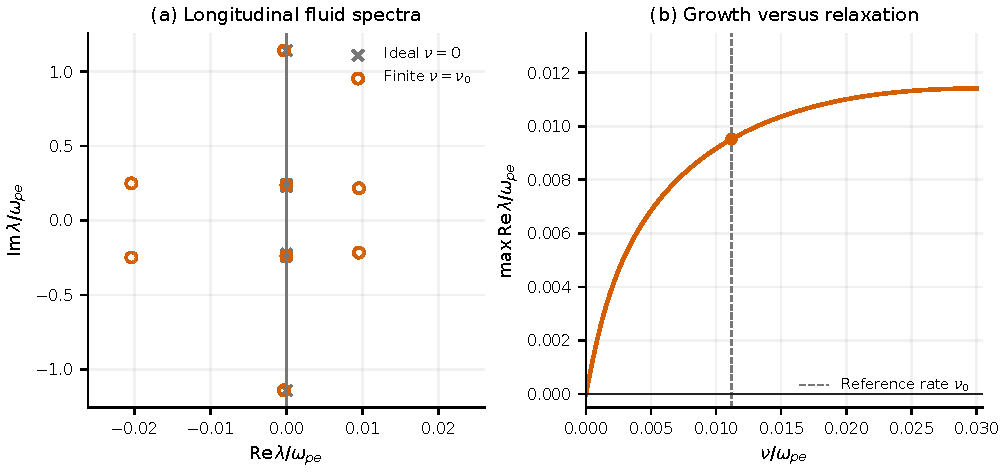
\includegraphics[width=\linewidth]{../figures/stability.pdf}
\caption{Homogeneous longitudinal test with $U/\sigma=1.2$ and
$k\sigma/\omega_{pe}=0.2$. Left: nonzero eigenvalues of the ideal and finite-rate
fluid systems; the static Gauss-constraint mode is excluded. Right: the
largest fluid growth rate as relaxation varies, with
$\nu_0/\omega_{pe}=1/(40\sqrt5)$ marked. The collisionless kinetic reference
has no growing longitudinal electrostatic mode by the Penrose proof above.
This comparison concerns the stated continuum closure, not an observed mode
in the original reconnection calculation.}
\label{fig:stability}
\end{figure}
